\documentclass{article}

\usepackage{amsmath,amsfonts,amssymb,amsthm}
\usepackage{listings,color}
\usepackage{graphicx}


% Opening
\title{Numerical Analysis HW5\\
Ch6 - 1,3,9 (pg178)\\
Ch7 - 1,3,5 (pg199)\\}
\author{Neal D. Nesbitt}

\begin{document}
\maketitle

\theoremstyle{definition}
\newtheorem{problem}{Problem}

\lstset{basicstyle=\ttfamily,
		language=Matlab,
		keywordstyle=\bf\color{blue},
		commentstyle=\it\color{magenta},
		identifierstyle=\bf
		}
		
\begin{problem}
	Employ fixed-point iteration to locate the root of
	\[ f(x) = \sin\left(\sqrt{x}\right)-x \]
	Use an initial guess of $x_{0}=0.5$ and iterate until $\epsilon_{a}\le 0.01\%$.\\
	Verify that the process is linearly convergent as described at the end of Sec 6.1.	
\end{problem}

If we can arrange a function such that $f(x)=$, simple fixed point iteration is taken by letting $x_{i+1}=f(x_{i})+x_{i}$. Since $f$ given above is already in this form, we can step through this method where
\[ x_{i+1} = f(x_{i}) + x_{i} = \sin\left( \sqrt{x_{i}} \right) \]
\begin{center}
	\begin{tabular}{|l c c c c|}
\hline
$i$	&	$x_{i}$	&	$\left| \epsilon_{a} \right|_{i}$	&	$\left| \epsilon_{a} \right|_{i}$	&	$\left| \epsilon_{t} \right|_{i}/\left| \epsilon_{t} \right|_{i-1}$\\ \hline
0	&	0.5000	&										&	34.95\%								&	0.4429\\
1	&	0.6496	&	23.03\%								&	15.48\%								&	0.3960\\
2	&	0.7215	&	9.97\%								&	6.13\%								&	0.3752\\
3	&	0.7509	&	3.92\%								&	2.30\%								&	0.3696\\
4	&	0.7621	&	1.47\%								&	0.85\%								&	0.3696\\
5	&	0.7678	&	0.21\%								&	0.10\%								&	0.1176\\
6	&	0.7683	&	0.07\%								&	0.04\%								&	0.4000\\
7	&	0.7685	&	0.03\%								&	0.01\%								&	0.2500\\
8	&	0.7686	&	0.01\%								&	0.00\%								&	0.0000\\
\hline
	\end{tabular}
\end{center}

\setcounter{problem}{2}
\begin{problem}
Determine the highest real root of
\[ f(x) = x^{3} - 6x^{2} + 11x - 6.1 \]
\begin{itemize}
\item Graphically
\item Using the Newton-Raphson method (three iterations, $x_{0}=3.5$)
\item Using the secant method (three iterations, $x_{i-1}=2.5$ and $x_{i}=3.5$)
\item Using the modified secant method (three iterations, $x_{i}=3.5$, $\delta = 0.01$)
\item Determine all the roots with MATLAB
\end{itemize}
\end{problem}

\paragraph{Graphically\\}
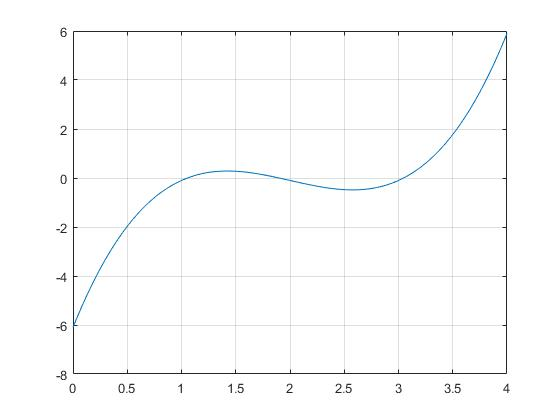
\includegraphics[width=\linewidth]{HW5-PolynomialGraph.jpg}
The graph suggests roots just above $x=1$, just below $x=2$, and just above $x=3$, making the root at $x\approx 3$ the largest.

\paragraph{Newton-Raphson}
\[ x_{i+1} = x_{i} - \frac{f(x_{i})}{f'(x_{i})} \]
\begin{center}
	\begin{tabular}{| l c c | c c |}
\hline
$i$	&	$x_{i}$	&	$| \epsilon_a |_{i}$	&	$f(x_{i})$	&	$f'(x_{i})$\\
\hline
0	&	3.5000	&							&	1.7750		&	5.7500\\ 
1	&	3.1913	&	9.6730\%				&	0.3994		&	3.2576\\ 
2	&	3.0687	&	3.9954\%				&	0.0519		&	2.4264\\ 
3	&	3.0473	&	0.7017\%				&	0.0015		&	2.2906\\
\hline
	\end{tabular}
\end{center}

\paragraph{Secant}
\[ x_{i+1} = x_{i} - \frac{f(x_{i})(x_{i-1}-x_{i})}{f(x_{i-1})-f(x_{i}))} \]
\begin{center}
	\begin{tabular}{| l c c | c |}
\hline
$i$	&	$x_{i}$	&	$| \epsilon_a |_{i}$	&	$f(x_{i})$\\
\hline
-1	&	2.5000	&							&	-0.4750\\
0	&	3.5000	&	28.57\%					&	1.7750\\
1	&	2.7111	&	29.0984\%				&	-0.4515\\
2	&	2.8711	&	5.5721\%				&	-0.3101\\
3	&	3.2219	&	10.8889\%				&	0.5024\\
\hline
	\end{tabular}
\end{center}

\paragraph{Modified Secant ($\delta=0.01$)}
\[ x_{i+1} = x_{i} - \frac{\delta x_{i}f(x_{i})}{f(x_{i}+\delta)-f(x_{i}))} \]
\begin{center}
	\begin{tabular}{| l c c | c c |}
\hline
$i$	&	$x_{i}$	&	$| \epsilon_a |_{i}$	&	$f(x_{i})$	&	$f(x_{i}+\delta x_{i})$	\\
\hline
0	&	3.5000	&							&	1.7750		&	1.9818\\
1	&	3.1996	&	9.3888\%				&	0.4267		&	0.5365\\
2	&	3.0753	&	4.0410\%				&	0.0681		&	0.1471\\
3	&	3.0488	&	0.8694\%				&	0.0049		&	0.0780\\
\hline
	\end{tabular}
\end{center}

\paragraph{MATLAB\\}
MATLAB's \verb|roots()| command tells us the 3 real roots are at $x=1.0544,1.8990,3.0467$.


\setcounter{problem}{8}
\begin{problem}
Employ the Newton-Raphson method to determine a real root for
\[ f(x) = -2 + 6x - 4x^{2} + 0.5x^{3} \]
using an initial guess of 4.5 and 4.43. Discuss and use graphical and analytical methods to explain any peculiarities in your results.
\end{problem}

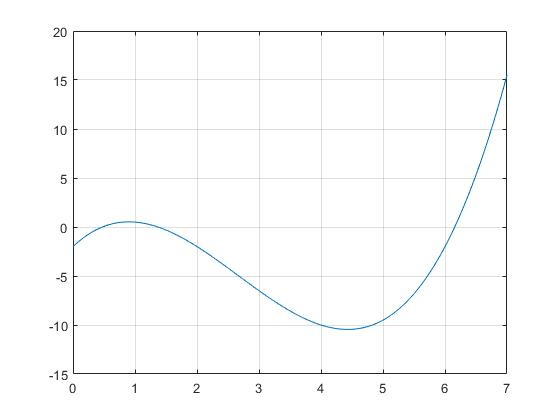
\includegraphics[width=\linewidth]{HW5-PolynomialGraph2.jpg}
Notice that we are very close to a local minimum for $x=4.5,4.43$. Then since the Newton-Raphson method uses the x intersection of the tangent line to pick its next point this throws us either wildly to the left or right depending on how close to this minimum we are. The closer we get, the farther it throws us away.
\[ f'(x_0)=0 \text{ and } f''(x_{0})>0 \implies \lim_{(x\to x_{0})^{-}}\frac{1}{f'(x)}=-\infty \text{ and } \lim_{(x\to x_{0})^{+}}\frac{1}{f'(x)}=+\infty \]

So if we look at the first few terms of the method to see this in action:
\[ x_{i+1} = x_{i} - \frac{f(x_{i})}{f'(x_{i})} \]
\begin{center}
	\begin{tabular}{| l c c | c c |}
\hline
$i$	&	$x_{i}$	&	$| \epsilon_a |_{i}$	&	$f(x_{i})$	&	$f'(x_{i})$\\
\hline
0	&	4.5		&							&	-10.4375	&	0.3750\\ 
1	&	32		&	86\%					&	12912		&	1315\\ 
2	&	22.5	&	43.6\%					&	3814.1		&	586.5\\ 
3	&	16		&	40.6\%					&	1121.9		&	262.6\\
\hline
	\end{tabular}
\end{center}

The first few terms of starting at $x=4.43$ have a order in the range of $10^{10}$ and don't even show up on the readout. 

All together, the $x=4.5$ gives the greatest root at a value of $x_{r}=6.1563$ after 11 iterations, and the starting point at $x=4.43$ shoots to the left and ends up giving back the least root of $x_{r}=0.4746$ after 25 iterations.

\setcounter{problem}{0}
\begin{problem}
Perform three iterations of the Newton-Raphson method to determine the root of Eq. (E7.1.1):
\[ \frac{dz}{dt} = v_{0}e^{-(c/m)t} - \frac{mg}{c}\left( 1 - e^{-(c/m)t} \right)\]
Use the parameter values from Example 7.1 ($g = 9.81 \text{ m/s}^{2}$, $z_{0} = 100 \text{ m}$, $v_{0} = 55 \text{ m/s}$, $m = 80 \text{ kg}$, and $c = 15 \text{ kg/s}$) along with an initial guess of $t = 3 \text{ s}$.
\end{problem}

\begin{center}
	\begin{tabular}{| l c c | c c |}
\hline
$i$	&	$t_{i}$	&	$| \epsilon_a |_{i}$	&	$f(t_{i})$	&	$f'(t_{i})$\\
\hline
0	&	3		&							&	8.8291		&	-11.4655\\ 
1	&	3.7701	&	20.4257\%				&	0.6078		&	-9.9240\\ 
2	&	3.8313	&	1.5986\%				&	0.0035		&	-9.8107\\ 
3	&	3.8317	&	0.0092\%				&	0.0000		&	-9.8100\\
\hline
	\end{tabular}
\end{center}

\setcounter{problem}{2}
\begin{problem}
Consider the following function:
\[ f(x) = 3 + 6x + 5x^{2} + 3x^{3} + 4x^{4} \]
Locate the minimum by finding the root of the derivative of this function. Use bisection with initial guesses of $x_{l} = -2$ and $x_{u} = 1$.
\end{problem}

Begin by taking the derivative.
\[ f'(x) = 6 + 5x +9x^{2} + 16x^{3} \]
Then using the bisect algorithm in MATLAB with the parameters given, we find the minimum to be at $x=-0.7791$ after 15 iterations with an absolute error of $\pm 0.0118$.


\setcounter{problem}{4}
\begin{problem}
Solve for the value of $x$ that maximizes $f(x)$ in Prob. 7.4 
\[ f(x) = -1.5x^{6} - 2x^{4} + 12x \]
using the golden-section search. Employ initial guesses of $x_{l} = 0$ and $x_{u} = 2$ and perform three iterations. 
\end{problem}

\begin{center}
	\begin{tabular}{| l | c c | c c | c c |c |}
\hline
$i$	&	$x_{l}$	&	$x_{u}$	&	$x_{1}$	&	$x_{2}$	&	$f(x_{1})$	&	$f(x_{2})$	&	$|\epsilon_{a}|$\\
\hline
0	&	0		&	2		&	1.2361	&	0.7639	&	4.8142		&	8.1879		&	61.8034\%\\
1	&	0		&	1.2361	&	0.7639	&	0.4721	&	8.1879		&	5.5496		&	38.1966\%\\
2	&	0.4721	&	1.2361	&	0.9443	&	0.7639	&	8.6778		&	8.1879		&	19.0983\%\\
3	&	0.7639	&	1.2361	&	1.0557	&	0.9443	&	8.1074		&	8.6778		&	11.8034\%\\
\hline
	\end{tabular}
\end{center}

\end{document}